
\section{\SCAMPLON{}}
\label{sec:proposal}

\SCAMPLON{}\footnote{\SCAMPLON{} stands as the contraction of \SCAMP{} and
  \CYCLON{}.} is a random peer sampling protocol inspired by both \SCAMP{} and
\CYCLON{}.  Firstly, \SCAMPLON{} reuses the joining process of \SCAMP{} to
incrementally build the network. While such network is not flawless, it has the
interesting property of logarithmically increasing the number of connections at
each join, compared to the global network size. Still, the newest members have
a small partial view size, and the oldest peers are more clustered. To
alleviates these issues, a periodic \CYCLON{}-like protocol takes place in
order to balance the partial views, using only neighbor-to-neighbor
interactions. This balancing concerns both the partial view sizes, and the
uniformity of chosen peers within them.

\SCAMPLON{} is adaptive, e.g., a peer with $2$ neighbors in its partial view
can exchange with a peer with $10$ neighbors. Ideally, the resulting size of
both partial views would be $6$ after the exchange. Yet, reaching this ideal
value in one cycle is difficult without the knowledge of each other's partial
view size. Instead of acquiring this knowledge, \SCAMPLON{} aims to converge to
the ideal value by averaging their view size over exchanges. Therefore, the
initiating peer $p_1$ sends $\left\lceil|\mathcal{P}_1|\over{2}\right\rceil$
members to the chosen peer $p_2$ (chosen by age). The latter sends back
$\left\lceil|\mathcal{P}_2|\over{2}\right\rceil$ members too. After the
receipt, both peers remove the sent members and add the received members. It
worth noting that \SCAMPLON{} uses a multiset as partial view. Therefore, a
neighbor can appear multiple times in a partial view, nonetheless, it
guarantees that the global number of connections after the process does not
change. The latter is crucial to ensure that each partial view tends to the
desired logarithmic size.

There exists a close relationship between \SCAMPLON{} and the proactive
aggregation protocol introduced
in~\cite{jelasity2004epidemic,montresor2004robust}. The latter states that,
under the assumption of a peer sampling sufficiently random, the mean value
$\mu$ and the variance $\sigma^2$ at a given cycle $i$ are:
\begin{center}
  $\mu_i = {1\over{|\mathcal{N}|}} \sum\limits_{x \in \mathcal{N}} a_{i,\,x}$
  \hfill
  $\sigma^2_i = {1\over{|\mathcal{N}|-1}}\sum\limits_{x \in \mathcal{N}}
  (a_{i,\,x} - \mu_i)^2$
\end{center}
where $a_{i,\,x}$ is the value held by Peer $p_x$ at cycle $i$. The estimated
variance must converge to $0$ over cycles. In other terms, the values tends to
be the same over cycles. In the \SCAMPLON{} case, the value $a_{i,\,x}$ is the
partial view size of Peer $p_x$ at cycle $i$. Indeed, each exchange from Peer
$p_1$ to Peer $p_2$ is an aggregation resulting to:
$|\mathcal{P}_1|\approx|\mathcal{P}_2|\approx{|\mathcal{P}_1| + |\mathcal{P}_2|
  \over{2}}$.
Furthermore, in the best case, each peer performs this exchange protocol
$1+Poisson(1)$ times per cycle, i.e., they initiate one and, in average,
receive one. However, the partial view sizes and the distribution of these
exchange protocol are linked together. Hence, the exchange distribution is
$1+Dist^t$, where the distribution $Dist$ is converging to $Poisson(1)$ over
time $t$.  This relation being established, we know that \SCAMPLON{} converges
exponentially fast. Furthermore, we know that each cycle decreases the variance
of the overall system at a rate between ${1\over{2}}$ and
$1\over{2\sqrt{\text{e}}}$.

\begin{asparadesc}
\item [Algorithm]\ref{algo:scamplon} shows the \SCAMPLON{} protocol running at
  each peer. It is divided between an active thread looping to update the
  partial view, and the events which provide the reactions to received
  messages. The functions which are not explicitly defined are the following:
  \begin{itemize}
  \item $incrementAge(view)$: increments the age of each elements in the view
    and returns the modified view.
  \item $getOldest(view)$: retrieves the oldest of peers contained in the view
  \item $getSample(view, \, size)$: returns a sample of the view containing
    $size$ elements.
  \item $replace(view,\,old,\,new)$: replaces in the view all occurrences of
    the $old$ element by the $new$ element and returns the modified view.
  \item $rand()$: generates a random number between 0 and 1.
  \end{itemize}
  A peer $o$ joining the network will reach a first contact peer. The latter
  will call Function $onSubs$ which spreads $(|\mathcal{P}|+c)$ copies of $o$
  inside the network, $c$ being a small constant value (typically lower that
  $3$). Then, each time a peer receives one of these message, assuming that
  this peer is not $o$, it has a probability $1\over{|\mathcal{P}|+1}$ to
  integrate $o$ in $\mathcal{P}$. Otherwise it forwards the copy to a random
  neighbor.  At this point, $o$ has $1$ neighbor in its partial view, and
  appears $(c+1)log(|\mathcal{N}|)$ times in partial views of other
  members. The active thread aims to balance the partial views. Each time
  Function $loop$ is called, the age of each element in $\mathcal{P}$ is
  incremented. Then, the oldest peer $q$ is chosen to exchange a subset of
  their partial view. If Peer $q$ cannot be reached (i.e. it crashed/left), it
  is removed from the partial view and the operation is repeated. Once the
  initiating peer $p$ found a reachable peer $q$, the former selects a sample
  of its partial view, excluding $q$ and including itself. The size of this
  sample is half of its partial view, with a minimum of one peer: the
  initiating peer. The answer of $q$ is of the exact same kind. Since peers can
  appear multiple times in $\mathcal{P}$, the exchanging peers may send
  references to the other peer, e.g., Peer $o$'s sample can contain references
  to $q$. Such sample, without further processing, would create self-loop
  ($q$'s partial view contains references to $q$). To alleviate this
  undesirable behavior, all occurrences of the other peer are replaced with the
  emitting peer.  Afterwards, both of them remove the sent sample from their
  view, remove the chosen neighbor, and add the received sample.
\end{asparadesc}


\begin{algorithm}
  
\small
\algrenewcommand{\algorithmiccomment}[1]{\hskip2em$\rhd$ #1}

\newcommand{\comment}[1]{$\rhd$ #1}


\algblockdefx[initially]{initially}{endInitially}
  [0] {\textbf{INITIALLY:}} 

\algblockdefx[act]{act}{endAct}
  [0] {\textbf{ACTIVE THREAD:}}

\algblockdefx[pas]{pas}{endPas}
  [0] {\textbf{PASSIVE THREAD:}}


\newcommand{\LINEFOR}[2]{%
  \algorithmicfor\ {#1}\ \algorithmicdo\ {#2} %
  }

\newcommand{\LINEIFTHEN}[2]{%
  \algorithmicif\ {#1}\ \algorithmicthen\ {#2} %
  }

\newcommand{\INDSTATE}[1][1]{\State\hspace{\algorithmicindent}}

\begin{algorithmic}[1]
  \Statex
  \initially
    \State $\mathcal{P} \leftarrow [\,]$;
    \hfill \comment{the partial view, sorted by age}
    \State $p$ ; \hfill \comment{identity of the local peer}
    \State $c \leftarrow 2$;
    \hfill \comment{additionnal connections when joining}

  \endInitially
  
  \act
    \Function{loop}{ } \hfill \comment{Every $\Delta$ time}
    \State $\mathcal{P} \leftarrow incrementAge(\mathcal{P})$;
    \State \textbf{let} $q \leftarrow getOldest(\mathcal{P})$;
    \State \textbf{let} $sample \leftarrow getSample(\mathcal{P}\setminus\left\{q\right\},\, \left \lceil{|\mathcal{P}|\over{2}} \right \rceil) \cup \left\{\langle p,\, 0 \rangle\right\}$;
    \State $sendTo(q,\, 'exchange',\, sample)$;
    \State \textbf{let} $sample'\leftarrow receiveFrom(q)$;
    \State $sample' \leftarrow replace(sample',\, p,\, q)$;
    \State $\mathcal{P} \leftarrow ((\mathcal{P} \setminus sample) \setminus \left\{ q \right\}) \cup sample'$;  \hfill \comment{update $\mathcal{P}$}
    \EndFunction
  \endAct
  
  \pas
    \Function{onExchange}{$o,\, sample$} \hfill \comment{$o: origin$}
    \State \textbf{let} $sample' \leftarrow getSample(\mathcal{P} ,\, \left\lceil |\mathcal{P}|\over{2} \right\rceil )$;
    \State $sendTo(o ,\, sample')$;
    \State $\mathcal{P} \leftarrow ((\mathcal{P} \setminus sample') \setminus \left\{ o \right\}) \cup sample$; \hfill \comment{update $\mathcal{P}$}
    \EndFunction
    \Statex
    \Function{onContact}{$o$} \hfill \comment{$o: origin$}
    \State \LINEFOR{\textbf{each} $q\in\mathcal{P}$}
    {$sendTo(q,\, 'fwdSubs',\, o)$;}
    \State \LINEFOR{$i \leftarrow 0$ \textbf{to} $c$}
    {\INDSTATE $sendTo(\mathcal{P}[\left\lfloor rand()*
        |\mathcal{P}|\right\rfloor],\, 'fwdSubs',\, o)$;}
    \EndFunction
    \Statex
    \Function{onFwdSubs}{$o$} \hfill \comment{$o: origin$}
    \If {$((rand() < (1 / (|\mathcal{P}|+1))) \wedge (o\not\in\mathcal{P}) 
      \wedge (o\neq p))$}
    \State $\mathcal{P} \leftarrow
    \mathcal{P}\cup \left\{\langle o,\, 0 \rangle\right\}$;
    \Else
    \State $sendTo(\mathcal{P}[\left\lfloor rand()*
      |\mathcal{P}|\right\rfloor],\, 'fwdSubs',\, o)$;
    \EndIf
    \EndFunction
  \endPas
  
\end{algorithmic}

  \caption{\label{algo:scamplon}The \SCAMPLON{} protocol.}
\end{algorithm}


\begin{asparadesc}
\item [Figure]~\ref{fig:scamplonexample} depicts an exchanging procedure
  between two peers $p_1$ and $p_2$. The initiating peer $p_1$ chooses its
  oldest neighbor $p_2$ to perform a neighborhood exchange. The former selects
  $\left\lceil{|\mathcal{P}_1|\over{2}}\right\rceil-1={4\over{2}}-1=1$ random
  peer among its neighborhood, here $\left\{p_1\right\}$. To this sample, it
  adds a reference to itself and sends the exchange message to $p_2$. The
  receipt of the message triggers the $onExchange$ event at Peer $p_2$. Hence,
  the latter chooses
  $\left\lceil{|\mathcal{P}_2|\over{2}}\right\rceil= {8\over{2}}=4$ random
  neighbors from its partial view to send back to Peer $p_1$. In this example
  it chooses $\{p_6,\,p_7,\,p_8,\,p_9\}$ and sends it to $p_1$. Afterwards,
  Peer $p_2$ cuts the connections to the peers it sent and creates new one with
  the received peer from $p_1$. Peer $p_1$ does the same, and additionally
  removes the connection chosen for the exchange, i.e., the connection to
  $p_2$. Afterwards, both partial view contains $6$ neighbors. Also, we can see
  that $p_1$ contains two times Peer $p_6$.
\end{asparadesc}



\begin{asparadesc}
\item [Algorithm]~\ref{algo:unreachable} shows the manner in which \SCAMPLON{}
  deals with crashes. Each time a neighbor is detected as crashed, the peer
  removes all occurrences of this neighbor in its partial view. The, for each
  removal, it doubles a reference to another of its neighbor with a probability
  of $1-{1\over{pSize}}$ where $pSize$ is the size of the partial view before
  the removals. This probability corresponds to the number of connections to
  reestablish in order to maintains the logarithmic complexity of partial view
  sizes. Indeed, on joining, a peer spreads $1+(c+1)log(|\mathcal{N}|)$
  connections in the network. On crash, it removes $2(c+1)log(|\mathcal{N}|)$
  connections: from the peers that reference the crashed peer, and from the
  crashed peer's partial view. Therefore, the peers that reference the crashed
  peer must reestablish one connection each, one peer excepted. Without global
  knowledge, each peer assumes that it could remove it itself. The probability
  of removal is ${1\over{pSize}}$. Thus, it will likely reestablish
  $(c+1)log(|\mathcal{N}|)-1$ connections globally after the execution of the
  algorithm by all peers referencing the crashed one.
\end{asparadesc}

\begin{algorithm}
  
\small
\SetKwProg{Function}{function}{}{}
\SetKwComment{tcp}{$\triangleright$~}{}
\DontPrintSemicolon
\LinesNumbered

\newcommand{\LET}[0]{\textbf{let}\xspace}
\newcommand{\FROM}[0]{\textup{\textbf{from}}\xspace}
\newcommand{\TO}[0]{\textup{\textbf{to}}\xspace}

\Function{\textup{onPeerDown ($q$)} \tcp*[f]{$q$: crashed/departed}} {
  \LET $occ \leftarrow 0$ \;

  \ForEach(\tcp*[f]{remove and count}) { $\langle n, age\rangle \in \mathcal{P}$ }  {
    \If {$n=q$} {
       $\mathcal{P} \leftarrow \mathcal{P}\setminus \{\langle n,\,age\rangle \}$ \;
       $occ \leftarrow occ + 1$ \;
    }
  }

  \For{$i$ \FROM $0$ \TO $occ$} {
    \tcp*[l]{probabilistically duplicates}

    \If{$\textup{rand( )}>{1\div{(|\mathcal{P}|+occ}})$} {
       \LET $\langle n,\,\_ \,\rangle \leftarrow
         \mathcal{P}[\left\lfloor \textup{rand( )}*|\mathcal{P}|\right\rfloor]$ \;
       $\mathcal{P} \leftarrow \mathcal{P} \uplus \left\{\langle n,\, 0\rangle\right\}$
    }
  }
}

\BlankLine

\Function{\textup{onArcDown($q$, $age$)} \tcp*[f]{$q$: arc arrival}} {
  $\mathcal{P} \leftarrow \mathcal{P}\setminus \{\langle q, age\rangle \}$ \;
  \tcp*[l]{systematically duplicates}
  \LET $\langle n, \_ \rangle \leftarrow
  \mathcal{P}[\left\lfloor \textup{rand( )}*|\mathcal{P}|\right\rfloor]$ \;
  $\mathcal{P} \leftarrow \mathcal{P} \uplus \left\{\langle n, 0\rangle\right\}$ \;

}

  \caption{\label{algo:unreachable}The crash handler.}
\end{algorithm}

Note that extending the algorithm to provide handshaking is not difficult: it
only requires to keep track of the neighbor from where the membership messages
arrived, and forward the answer to this neighbor accordingly. Also, there are
few optimization concerning the establishments of connections. For instance,
when a peer $p$ starts an exchange with $q$, and $q$ has $p$ in its partial
view, instead of inverting the link between $p$ and $q$, and $q$ and $p$,
\SCAMPLON{} does not change them. Another optimization concerns a peer having a
neighbor multiple times in its partial view. While \SCAMPLON{} keeps such
information in its partial view, only one connection per neighbor is truly
necessary.

\begin{figure*}
  \centering
  
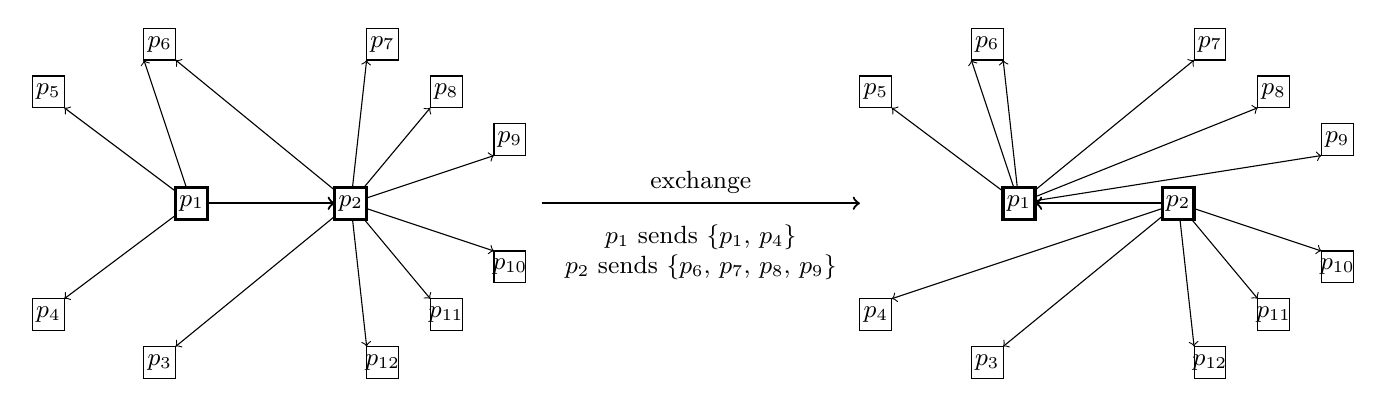
\begin{tikzpicture}[scale=1.15]
  \small

  \draw[->] (0pt,  0pt) -- ( -40pt,  30pt );
  \draw[->] (0pt,  0pt) -- ( -40pt, -30pt );
  \draw[->] (0pt,  0pt) -- ( -15pt,  45pt );

  \draw[->, thick] (0pt, 0pt) -- (45pt, 0pt);
  \draw[->] (50pt, 0pt) -- (-5pt, -45pt);
  \draw[->] (50pt, 0pt) -- (-5pt, 45pt);

  \draw[fill=white, very thick](0pt, 0pt)
  node{$p_1$}+(-5pt,-5pt)rectangle +(5pt,5pt);
  \draw[fill=white] (-10pt, 50pt)node{$p_6$} +(-5pt,-5pt) rectangle +(5pt,5pt);
  \draw[fill=white] (-45pt, 35pt)node{$p_5$} +(-5pt,-5pt) rectangle +(5pt,5pt);
  \draw[fill=white] (-45pt,-35pt)node{$p_4$} +(-5pt,-5pt) rectangle +(5pt,5pt);
  \draw[fill=white] (-10pt,-50pt)node{$p_3$} +(-5pt,-5pt) rectangle +(5pt,5pt);

  \begin{scope}[shift={(50pt,0pt)}]
  \draw[->] (0pt, 0pt) -- (   5pt, -45pt );
  \draw[->] (0pt, 0pt) -- ( 45pt, -15pt );
  \draw[->] (0pt, 0pt) -- ( 25pt, -30pt );
  \draw[->] (0pt, 0pt) -- (  25pt, 30pt );
  \draw[->] (0pt, 0pt) -- (  45pt, 15pt );
  \draw[->] (0pt, 0pt) -- (   5pt, 45pt );

  \draw[fill=white, very thick] (0pt, 0pt)
  node{$p_2$} +(-5pt,-5pt) rectangle +(5pt,5pt);
  \draw[fill=white] ( 10pt, 50pt)node{$p_{7}$}+(-5pt,-5pt)rectangle+(5pt,5pt);
  \draw[fill=white] ( 30pt, 35pt)node{$p_{8}$}+(-5pt,-5pt)rectangle+(5pt,5pt);
  \draw[fill=white] ( 50pt, 20pt)node{$p_{9}$}+(-5pt,-5pt)rectangle+(5pt,5pt);

  \draw[fill=white] ( 50pt,-20pt)node{$p_{10}$}+(-5pt,-5pt)rectangle+(5pt,5pt);
  \draw[fill=white] ( 30pt,-35pt)node{$p_{11}$}+(-5pt,-5pt)rectangle+(5pt,5pt);
  \draw[fill=white] ( 10pt,-50pt)node{$p_{12}$}+(-5pt,-5pt)rectangle+(5pt,5pt);
  \end{scope}
 

  \draw[->,thick] (110pt, 0pt) --node[anchor=south]{exchange}
  node[anchor=north, align=center]{ \ \\
    $p_1$ sends $\left\{p_1,\,p_4\right\}$\\
  $p_2$ sends $\left\{p_6,\,p_7,\,p_8,\,p_9\right\}$}
  (210pt, 0pt);

  \begin{scope}[shift={(260pt, 0pt)}]
  \draw[->] (0pt, 0pt) -- ( -40pt,  30pt );
  \draw[->] (0pt, 0pt) -- ( -15pt,  45pt );
  \draw[->] (0pt, 0pt) -- (  -5pt,  45pt );


  \draw[<-, thick] (5pt, 0pt) -- (50pt, 0pt);
  \draw[->] (50pt, 0pt) -- (-5pt, -45pt);
  \draw[->] (50pt, 0pt) -- (-40pt, -30pt);
  \draw[->] (0pt, 0pt) -- (  55pt, 45pt );
  \draw[->] (0pt, 0pt) -- ( 95pt,  15pt );
  \draw[->] (0pt, 0pt) -- ( 75pt,  30pt );

  \draw[fill=white, very thick](0pt, 0pt)
  node{$p_1$}+(-5pt,-5pt)rectangle +(5pt,5pt);
  \draw[fill=white] (-10pt, 50pt)node{$p_6$} +(-5pt,-5pt) rectangle +(5pt,5pt);
  \draw[fill=white] (-45pt, 35pt)node{$p_5$} +(-5pt,-5pt) rectangle +(5pt,5pt);
  \draw[fill=white] (-45pt,-35pt)node{$p_4$} +(-5pt,-5pt) rectangle +(5pt,5pt);
  \draw[fill=white] (-10pt,-50pt)node{$p_3$} +(-5pt,-5pt) rectangle +(5pt,5pt);

  \begin{scope}[shift={(50pt,0pt)}]
  \draw[->] (0pt, 0pt) -- (  25pt, -30pt );
  \draw[->] (0pt, 0pt) -- (  45pt, -15pt );
  \draw[->] (0pt, 0pt) -- (   5pt, -45pt );

  \draw[fill=white, very thick] (0pt, 0pt)
  node{$p_2$} +(-5pt,-5pt) rectangle +(5pt,5pt);
  \draw[fill=white] ( 10pt, 50pt)node{$p_{7}$}+(-5pt,-5pt)rectangle+(5pt,5pt);
  \draw[fill=white] ( 30pt, 35pt)node{$p_{8}$}+(-5pt,-5pt)rectangle+(5pt,5pt);
  \draw[fill=white] ( 50pt, 20pt)node{$p_{9}$}+(-5pt,-5pt)rectangle+(5pt,5pt);

  \draw[fill=white] ( 50pt,-20pt)node{$p_{10}$}+(-5pt,-5pt)rectangle+(5pt,5pt);
  \draw[fill=white] ( 30pt,-35pt)node{$p_{11}$}+(-5pt,-5pt)rectangle+(5pt,5pt);
  \draw[fill=white] ( 10pt,-50pt)node{$p_{12}$}+(-5pt,-5pt)rectangle+(5pt,5pt);
  \end{scope}

  \end{scope}
  
\end{tikzpicture}
  \caption{\label{fig:scamplonexample} A round of exchange between two peers
    using \SCAMPLON{}. In this case, Peer $p_1$ initiates an exchange with its
    oldest neighbor $p_2$ (for simplicity sake, only the partial view of the
    peers involved in the exchange are explicitly drawn). The network on the
    left shows the network before the exchange, and the network on the right
    shows the network after the exchange. After the exchange of peers chosen at
    random, both peers $p_1$ and $p_2$ have a partial view size of $6$.}
\end{figure*}

To summarize, \SCAMPLON{} provides the best of its parents:
\begin{inparaenum}[(i)]
\item a logarithmically increasing partial view size compared to the global
  network size,
\item a constant complexity to establish the connections,
\item an exponentially fast convergence to a random graph.
\end{inparaenum}
Providing these three properties, \SCAMPLON{} improves the state-of-the-art
approaches~\cite{ganesh2001scamp,voulgaris2005cyclon} in the traditional
connection set-up. Furthermore, the improvement becomes crucial in the context
of three-way handshake connection set-up.  The latter becomes increasingly
important with the appearance of technologies allowing peer-to-peer within
modern web browsers.  The next section aims to demonstrate experimentally the
behavior of \SCAMPLON{}. In particular, it aims to highlight the aforementioned
properties.


%%% Local Variables:
%%% mode: latex
%%% TeX-master: "../paper"
%%% End:
